%%%%%%%%%%%%%%%%%%%%%%%%%%%%%%%%%%%%%%%%%
% Awesome Resume/CV
% XeLaTeX Template
% Version 1.2 (27/3/2017)
%
% This template has been downloaded from:
% http://www.LaTeXTemplates.com
%
% Original author:
% Claud D. Park (posquit0.bj@gmail.com) with modifications by 
% Vel (vel@latextemplates.com)
%
% License:
% CC BY-NC-SA 3.0 (http://creativecommons.org/licenses/by-nc-sa/3.0/)
%
% Important note:
% This template must be compiled with XeLaTeX, the below lines will ensure this
%!TEX TS-program = xelatex
%!TEX encoding = UTF-8 Unicode
%
%%%%%%%%%%%%%%%%%%%%%%%%%%%%%%%%%%%%%%%%%

%----------------------------------------------------------------------------------------
%	PACKAGES AND OTHER DOCUMENT CONFIGURATIONS
%----------------------------------------------------------------------------------------

\documentclass[11pt, a4paper]{awesome-cv} % A4 paper size by default, use 'letterpaper' for US letter

\geometry{left=2cm, top=1.5cm, right=2cm, bottom=2cm, footskip=.5cm} % Configure page margins with geometry

\fontdir[fonts/] % Specify the location of the included fonts

% Color for highlights
\colorlet{awesome}{awesome-red} % Default colors include: awesome-emerald, awesome-skyblue, awesome-red, awesome-pink, awesome-orange, awesome-nephritis, awesome-concrete, awesome-darknight
%\definecolor{awesome}{HTML}{CA63A8} % Uncomment if you would like to specify your own color

% Colors for text - uncomment and modify
%\definecolor{darktext}{HTML}{414141}
%\definecolor{text}{HTML}{414141}
%\definecolor{graytext}{HTML}{414141}
%\definecolor{lighttext}{HTML}{414141}

\renewcommand{\acvHeaderSocialSep}{\quad\textbar\quad} % If you would like to change the social information separator from a pipe (|) to something else

%----------------------------------------------------------------------------------------
%	PERSONAL INFORMATION
%	Comment any of the lines below if they are not required
%----------------------------------------------------------------------------------------

\name{Claud D.}{Park}
\address{246-1002, Gwangmyeongmayrouge Apt. 86, Cheongna lime-ro, Seo-gu, Incheon-si, 404-180, Rep. of KOREA}
\mobile{(+82) 10-9030-1843}

\email{posquit0.bj@gmail.com}
\homepage{www.posquit0.com}
\github{posquit0}
\linkedin{posquit0}
%\skype{skypeid}
%\stackoverflow{SOid}{SOname}
%\twitter{@twit}
%\linkedin{linkedin name}
%\reddit{reddit account}
%\xing{xing name}
%\extrainfo{test} % Other text you want to include on this line

\position{Software Engineer{\enskip\cdotp\enskip}Security Expert} % Your expertise/fields
\quote{``Make the change that you want to see in the world."} % A quote or statement

\makecvfooter{\today}{Claud D. Park~~~·~~~Résumé}{\thepage} % Specify the letter footer with 3 arguments: (<left>, <center>, <right>), leave any of these blank if they are not needed

%----------------------------------------------------------------------------------------

\begin{document}

\makecvheader % Print the header

%----------------------------------------------------------------------------------------
%	CV/RESUME CONTENT
%	Each section is imported separately, open each file in turn to modify content
%----------------------------------------------------------------------------------------

%----------------------------------------------------------------------------------------
%	SECTION TITLE
%----------------------------------------------------------------------------------------

\cvsection{Education}

%----------------------------------------------------------------------------------------
%	SECTION CONTENT
%----------------------------------------------------------------------------------------

\begin{cventries}

%------------------------------------------------

\cventry
{B.S. in Computer Science and Engineering} % Degree
{POSTECH(Pohang University of Science and Technology)} % Institution
{Pohang, S.Korea} % Location
{Mar. 2010 - PRESENT} % Date(s)
{ % Description(s) bullet points
\begin{cvitems}
\item {Got a Chun Shin-Il Scholarship which is given to promising students in CSE Dept.}
\end{cvitems}
}

%------------------------------------------------

\end{cventries}
%----------------------------------------------------------------------------------------
%	SECTION TITLE
%----------------------------------------------------------------------------------------

\cvsection{Skills}

%----------------------------------------------------------------------------------------
%	SECTION CONTENT
%----------------------------------------------------------------------------------------

\begin{cvskills}

%------------------------------------------------

\cvskill
{Programming} % Category
{Python, C/C++, Scala, JAVA, Node.JS, OCaml, LaTeX} % Skills

%------------------------------------------------

\cvskill
{Web} % Category
{Django with Python, Express with Node.JS, HTML5, LESS} % Skills

%------------------------------------------------

\cvskill
{Languages} % Category
{Korean, English, Japanese, Chinese} % Skills

%------------------------------------------------

\end{cvskills}
%----------------------------------------------------------------------------------------
%	SECTION TITLE
%----------------------------------------------------------------------------------------

\cvsection{Experience}

%----------------------------------------------------------------------------------------
%	SECTION CONTENT
%----------------------------------------------------------------------------------------

\begin{cventries}

%------------------------------------------------

\cventry
{Software Engineer \& Security Researcher (Compulsory Military Service)} % Job title
{R.O.K Cyber Command, MND} % Organization
{Seoul, S.Korea} % Location
{Aug. 2014 - Exp. Apr. 2016} % Date(s)
{ % Description(s) of tasks/responsibilities
\begin{cvitems}
\item {Implemented a military cooperation system which is web based real time messenger in Scala on Lift.}
\item {Improved functionality on military command and control system for incident response with Java Servlet.}
\item {Lead engineer on agent-less backtracking system that can discover client device's fingerprint(including public and private IP) independently of the Proxy, VPN and NAT.}
\end{cvitems}
}

%------------------------------------------------    

\cventry
{Game Developer Intern at Global Internship Program} % Job title
{NEXON} % Organization
{Seoul, S.Korea \& LA, U.S.A} % Location
{Jan. 2013 - Feb. 2013} % Date(s)
{ % Description(s) of tasks/responsibilities
\begin{cvitems}
\item {Developed in Cocos2d-x an action puzzle game(Dragon Buster) targeting U.S. market. Implemented API server which is communicating with game client and In-App Store, along with two other team members who wrote the game logic, designed game graphics.}
\item {Won the 2nd prize in final evaluation.}
\end{cvitems}
}

%------------------------------------------------

\cventry
{Researcher for <Detecting video’s torrents using image similarity algorithms>} % Job title
{Undergraduate Research, Computer Vision Lab(Prof. Bohyung Han)} % Organization
{Pohang, S.Korea} % Location
{Sep. 2012 - Feb. 2013} % Date(s)
{ % Description(s) of tasks/responsibilities
\begin{cvitems}
\item {Researched means of retrieving a corresponding video based on image contents using image similarity algorithm.}
\item {Implemented prototype that users can obtain torrent magnet links of corresponding video relevant to an image on web site.}
\end{cvitems} 
}

%------------------------------------------------

\cventry
{Software Engineer Trainee} % Job title
{Software Maestro (funded by Korea Ministry of Knowledge and Economy)} % Organization
{Seoul, S.Korea} % Location
{Jul. 2012 - Jun. 2013} % Date(s)
{ % Description(s) of tasks/responsibilities
\begin{cvitems}
\item {Performed research memory management strategies of OS and implemented in Python an interactive simulator for Linux kernel memory management.}
\end{cvitems}
}

%------------------------------------------------

\cventry
{Software Engineer} % Job title
{ShitOne Corp. (Start-up company)} % Organization
{Seoul, S.Korea} % Location
{Dec. 2011 - Feb. 2012} % Date(s)
{ % Description(s) of tasks/responsibilities
\begin{cvitems}
\item {Developed a proxy drive smartphone application which connects proxy driver and customer. Implemented overall Android application logic and wrote API server for community service, along with lead engineer who designed bidding protocol on raw socket and implemented API server for bidding.}
\end{cvitems}
}

%------------------------------------------------

\cventry
{Freelance Penetration Tester} % Job title
{SAMSUNG Electronics} % Organization
{S.Korea} % Location
{Sep. 2013, Mar. 2011 - Oct. 2011} % Date(s)
{ % Description(s) of tasks/responsibilities
\begin{cvitems}
\item {Conducted penetration testing on SAMSUNG KNOX, which is solution for enterprise mobile security.}
\item {Conducted penetration testing on SAMSUNG Smart TV.}
\end{cvitems}
}

%------------------------------------------------

\end{cventries}

\newpage % Force a new page for looks

%----------------------------------------------------------------------------------------
%	SECTION TITLE
%----------------------------------------------------------------------------------------

\cvsection{Extracurricular Activity}

%----------------------------------------------------------------------------------------
%	SECTION CONTENT
%----------------------------------------------------------------------------------------

\begin{cventries}

%------------------------------------------------

\cventry
{Core Member} % Affiliation/role
{B10S (B1t 0n the Security, Underground hacker team)} % Organization/group
{S.Korea} % Location
{Nov. 2011 - PRESENT} % Date(s)
{ % Description(s) of experience/contributions/knowledge
\begin{cvitems}
\item {Gained expertise in penetration testing areas, especially targeted on web application and software.}
\item {Participated on a lot of hacking competition and won a good award.}
\item {Held several hacking competitions non-profit, just for fun.}
\end{cvitems}
}

%------------------------------------------------

\cventry
{Member} % Affiliation/role
{WiseGuys (Hacking \& Security research group)} % Organization/group
{S.Korea} % Location
{Jun. 2012 - PRESENT} % Date(s)
{ % Description(s) of experience/contributions/knowledge
\begin{cvitems}
\item {Gained expertise in hardware hacking areas from penetration testing on several devices including wireless router, smartphone, CCTV and set-top box.}
\item {Trained wannabe hacker about hacking technique from basic to advanced and ethics for white hackers by hosting annual Hacking Camp.}
\end{cvitems}
}

%------------------------------------------------

\cventry
{Core Member \& President at 2013} % Affiliation/role
{PoApper (Developers' Network of POSTECH)} % Organization/group
{Pohang, S.Korea} % Location
{Jun. 2010 - PRESENT} % Date(s)
{ % Description(s) of experience/contributions/knowledge
\begin{cvitems}
\item {Reformed the society focusing on software engineering and building network on and off campus.}
\item {Proposed various marketing and network activities to raise awareness.}
\end{cvitems}
}

%------------------------------------------------

\cventry
{Member} % Affiliation/role
{PLUS (Laboratory for UNIX Security in POSTECH)} % Organization/group
{Pohang, S.Korea} % Location
{Sep. 2010 - Oct. 2011} % Date(s)
{ % Description(s) of experience/contributions/knowledge
\begin{cvitems}
\item {Gained expertise in hacking \& security areas, especially about internal of operating system based on UNIX and several exploit techniques.}
\item {Participated on several hacking competition and won a good award.}
\item {Conducted periodic security checks on overall IT system as a member of POSTECH CERT.}
\item {Conducted penetration testing commissioned by national agency and corporation.}
\end{cvitems}
}

%------------------------------------------------

\cventry
{Member} % Affiliation/role
{MSSA (Management Strategy Club of POSTECH)} % Organization/group
{Pohang, S.Korea} % Location
{Sep. 2013 - PRESENT} % Date(s)
{ % Description(s) of experience/contributions/knowledge
\begin{cvitems}
\item {Gained knowledge about several business field like Management, Strategy, Financial and marketing from group study.}
\item {Gained expertise in business strategy areas and inisght for various industry from weekly industry analysis session.}
\end{cvitems}
}

%------------------------------------------------

\end{cventries}
%----------------------------------------------------------------------------------------
%	SECTION TITLE
%----------------------------------------------------------------------------------------

\cvsection{Honors \& Awards}

%----------------------------------------------------------------------------------------
%	INTERNATIONAL SUBSECTION
%----------------------------------------------------------------------------------------

\cvsubsection{International}

%------------------------------------------------

\begin{cvhonors}

%------------------------------------------------

\cvhonor
{Finalist} % Award
{DEFCON 22nd CTF Hacking Competition World Final} % Event
{Las Vegas, U.S.A} % Location
{2014} % Date(s)

%------------------------------------------------

\cvhonor
{Finalist} % Award
{DEFCON 21st CTF Hacking Competition World Final} % Event
{Las Vegas, U.S.A} % Location
{2013} % Date(s)

%------------------------------------------------

\cvhonor
{Finalist} % Award
{DEFCON 19th CTF Hacking Competition World Final} % Event
{Las Vegas, U.S.A} % Location
{2011} % Date(s)

%------------------------------------------------

\cvhonor
{6th Place} % Award
{SECUINSIDE Hacking Competition World Final} % Event
{Seoul, S.Korea} % Location
{2012} % Date(s)

%------------------------------------------------

\end{cvhonors}

%----------------------------------------------------------------------------------------
%	DOMESTIC SUBSECTION
%----------------------------------------------------------------------------------------

\cvsubsection{Domestic}

%------------------------------------------------

\begin{cvhonors}

%------------------------------------------------

\cvhonor
{3rd Place} % Award
{WITHCON Hacking Competition Final} % Event
{Seoul, S.Korea} % Location
{2015} % Date(s)

%------------------------------------------------

\cvhonor
{Silver Prize} % Award
{KISA HDCON Hacking Competition Final} % Event
{Seoul, S.Korea} % Location
{2013} % Date(s)

%------------------------------------------------

\cvhonor
{2nd Award} % Award
{HUST Hacking Festival} % Event
{S.Korea} % Location
{2013} % Date(s)

%------------------------------------------------

\cvhonor
{3rd Award} % Award
{HUST Hacking Festival} % Event
{S.Korea} % Location
{2010} % Date(s)


%------------------------------------------------

\cvhonor
{3rd Award} % Award
{Holyshield 3rd Hacking Festival} % Event
{S.Korea} % Location
{2012} % Date(s)

%------------------------------------------------

\cvhonor
{2nd Award} % Award
{Holyshield 3rd Hacking Festival} % Event
{S.Korea} % Location
{2011} % Date(s)

%------------------------------------------------

\cvhonor
{5th Place} % Award
{PADOCON Hacking Competition Final} % Event
{Seoul, S.Korea} % Location
{2011} % Date(s)

%------------------------------------------------

\end{cvhonors}
%%%%%%%%%%%%%%%%%%%%%%%%%%%%%%%%%%%%%%%%%
% Fancyslides Presentation
% LaTeX Template
% Version 1.0 (30/6/13)
%
% This template has been downloaded from:
% http://www.LaTeXTemplates.com
%
% The Fancyslides class was created by:
% Paweł Łupkowski (pawel.lupkowski@gmail.com)
%
% License:
% CC BY-NC-SA 3.0 (http://creativecommons.org/licenses/by-nc-sa/3.0/)
%
%%%%%%%%%%%%%%%%%%%%%%%%%%%%%%%%%%%%%%%%%

%----------------------------------------------------------------------------------------
%	PACKAGES AND OTHER DOCUMENT CONFIGURATIONS
%----------------------------------------------------------------------------------------

\documentclass{fancyslides}

\usepackage[utf8]{inputenc} % Allows the usage of non-english characters
\usepackage{times} % Use the Times font
\usepackage{booktabs} % Allows the use of \toprule, \midrule and \bottomrule in tables
\graphicspath{{images/}} % Location of the slide background and figure files

% Beamer options - do not change
\usetheme{default}
\setbeamertemplate{navigation symbols}{} % Disable the slide navigation buttons on the bottom of each slide
\setbeamercolor{structure}{fg=\yourowntexcol} % Define the color of titles and fixed text elements (e.g. bullet points)
\setbeamercolor{normal text}{fg=\yourowntexcol} % Define the color of text in the presentation

%------------------------------------------------
% COLORS
% The following colors are predefined in this class: white, black, gray, blue, green and orange

% Define your own color as follows:
%\definecolor{pink}{rgb}{156,0,151}

\newcommand{\structureopacity}{0.75} % Opacity (transparency) for the structure elements (boxes and circles)

\newcommand{\strcolor}{blue} % Set the color of structure elements (boxes and circles)
\newcommand{\yourowntexcol}{white} % Set the text color

%----------------------------------------------------------------------------------------
%	TITLE SLIDE
%----------------------------------------------------------------------------------------

\newcommand{\titlephrase}{A LONG AND COMPLICATED PRESENTATION TITLE} % Presentation title
\newcommand{\name}{John Smith} % Presenter's name
\newcommand{\affil}{UCLA} % Presenter's institution
\newcommand{\email}{john@LaTeXTemplates.com} % Presenter's email address

\begin{document}

\startingslide % This command inserts the title slide as the first slide

%----------------------------------------------------------------------------------------
%	PRESENTATION SLIDES
%----------------------------------------------------------------------------------------

\fbckg{1.jpg} % Slide background image
\begin{frame}
\pointedsl{main point} % Text in this environment is printed in a circle and will be made large and uppercase - if you need to fit more text in you can reduce the font size within the \pointedsl{} bracket as usual, e.g. \pointedsl{\large smaller main point}
\end{frame}

%------------------------------------------------

\fbckg{2.jpg} % Slide background image
\begin{frame}
\framedsl{explained clearly with more text} % Text in this environment will be made large, uppercase and will wrap multiple lines
\end{frame}

%------------------------------------------------

\fbckg{2.jpg} % Slide background image
\begin{frame}
\itemized{ % This environment simply prints a series of bullet points
\item or as a list containing multiple points
\item alternatively, you may want a few main points appearing one by one\ldots
}
\end{frame}

%------------------------------------------------

\fbckg{2.jpg} % Slide background image
\begin{frame}
\framedsl{\pitem{First point} \pitem{Second point} \fitem{Third point}} % Text in \pitem commands will be printed one after another on separate slides until all are displayed
\end{frame}

%------------------------------------------------

\fbckg{2.jpg} % Slide background image
\begin{frame}
\misc{ % Anything can be placed inside the \misc{} command
\Huge
Numbered list:
\begin{enumerate}
\centering
\item First item
\item Second item
\item Third item
\end{enumerate}
}
\end{frame}

%------------------------------------------------

\fbckg{2.jpg} % Slide background image
\begin{frame}
\misc{ % Anything can be placed inside the \misc{} command
Tables can be included with the \texttt{\textbackslash misc\{\}} command:
\begin{table}[h]
\begin{tabular}{l l l}
\toprule
\textbf{Treatments} & \textbf{Response 1} & \textbf{Response 2}\\
\midrule
Treatment 1 & 0.0003262 & 0.562 \\
Treatment 2 & 0.0015681 & 0.910 \\
Treatment 3 & 0.0009271 & 0.296 \\
\bottomrule
\end{tabular}
\end{table}
}
\end{frame}

%------------------------------------------------

\fbckg{2.jpg} % Slide background image
\begin{frame}
\misc{ % Anything can be placed inside the \misc{} command
Figures can also be included with the \texttt{\textbackslash misc\{\}} command:
\begin{figure}[h]

\includegraphics[width=0.4\linewidth]{placeholder}
\end{figure}
}
\end{frame}

%------------------------------------------------

\fbckg{1.jpg} % Slide background image
\begin{frame}
\thankyou % Inserts a thank you slide
\end{frame}

%------------------------------------------------

\fbckg{blank} % A blank background can be used instead of an image
\begin{frame}
\sources{ % An environment for giving credit for slide backgrounds, images will need to be scaled down if there are more than two
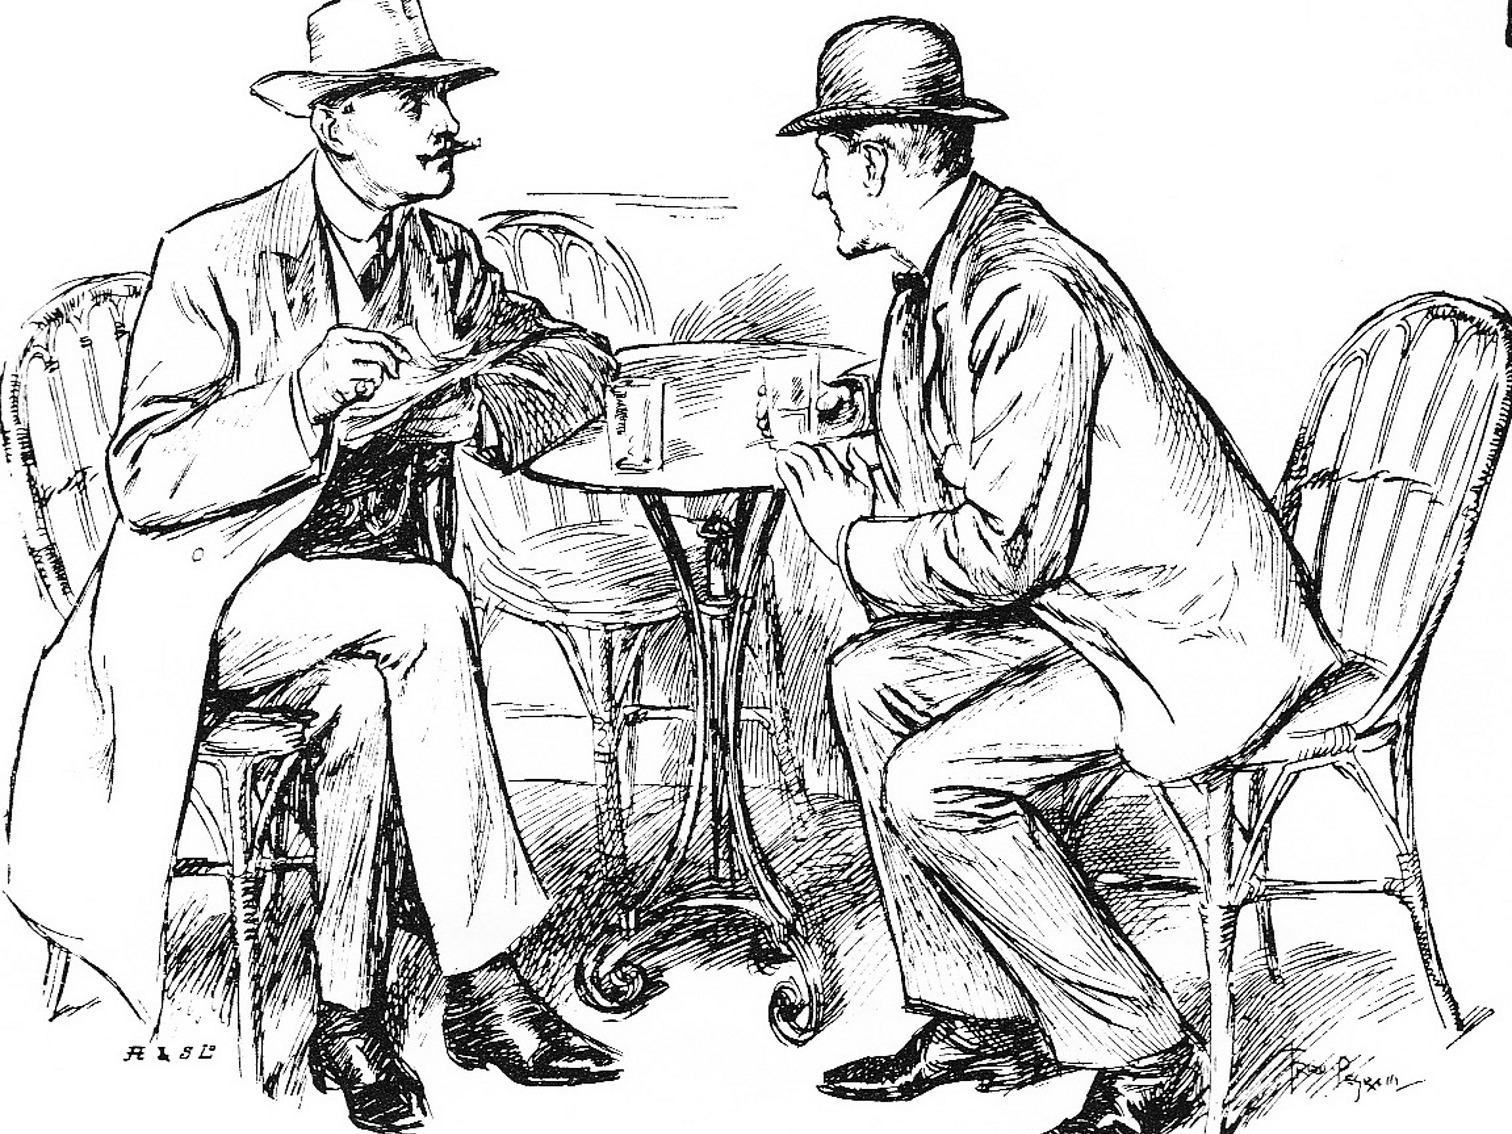
\includegraphics[scale=0.048]{1.jpg} \ flickr/lovelornpoets\\
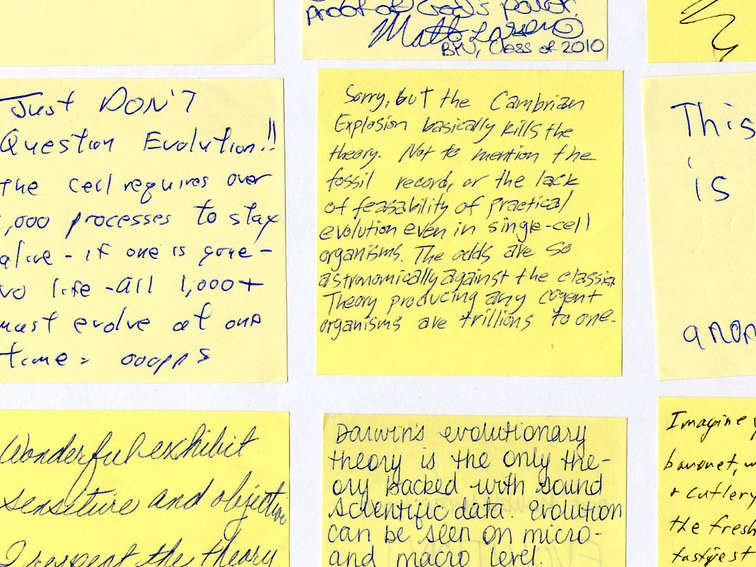
\includegraphics[scale=0.2]{2.jpg} \ flickr/apsmuseum
}
\end{frame}

%----------------------------------------------------------------------------------------

\end{document}

%----------------------------------------------------------------------------------------
%	SECTION TITLE
%----------------------------------------------------------------------------------------

\cvsection{Writing}

%----------------------------------------------------------------------------------------
%	SECTION CONTENT
%----------------------------------------------------------------------------------------

\begin{cventries}

%------------------------------------------------

\cventry
{Founder \& Writer} % Role
{A Guide for Developers in Start-up} % Title
{Facebook Page} % Location
{Jan. 2015 - PRESENT} % Date(s)
{ % Description(s)
\begin{cvitems}
\item {Drafted daily news for developers in Korea about IT technologies, issues about start-up.}
\end{cvitems}
}

%------------------------------------------------

\cventry
{Undergraduate Student Reporter} % Role
{AhnLab} % Title
{S.Korea} % Location
{Oct. 2012 - Jul. 2013} % Date(s)
{ % Description(s)
\begin{cvitems}
\item {Drafted reports about IT trends and Security issues on AhnLab Company magazine.}
\end{cvitems}
}

%------------------------------------------------

\end{cventries}
%----------------------------------------------------------------------------------------
%	SECTION TITLE
%----------------------------------------------------------------------------------------

\cvsection{Program Committees}

%----------------------------------------------------------------------------------------
%	SECTION CONTENT
%----------------------------------------------------------------------------------------

\begin{cvhonors}

%------------------------------------------------

\cvhonor
{Organizer \& Co-director} % Position
{1st POSTECH Hackathon} % Committee
{S.Korea} % Location
{2013} % Date(s)
    
%------------------------------------------------

\cvhonor
{Staff} % Position
{7th Hacking Camp} % Committee
{S.Korea} % Location
{2012} % Date(s)

%------------------------------------------------

\cvhonor
{Problem Writer} % Position
{1st Hoseo University Teenager Hacking Competition} % Committee
{S.Korea} % Location
{2012} % Date(s)

%------------------------------------------------

\cvhonor
{Staff \& Problem Writer} % Position
{JFF(Just for Fun) Hacking Competition} % Committee
{S.Korea} % Location
{2012} % Date(s)

%------------------------------------------------

\end{cvhonors}

%----------------------------------------------------------------------------------------

\end{document}
